%-- Add sections and your outline will be created automatically --%
\subsection{The lock--exchange}

% Frame starts a new slide
\begin{frame}
    \frametitle{The lock--exchange}
\begin{itemize}
\item Fluids of different densities (temperature) separated by a barrier. As the barrier is removed, the denser fluid
  collapses under the lighter.
\item Boussinesq flow, control volume discretisation, mesh adaptivity
\item Run time: 10 min.
\end{itemize}

\begin{figure}
\centering

\includegraphics[width=0.45\textwidth]{./lock_exchange/le_basic_0_T}
\caption{Lock-exchange initial temperature (colour) distribution.}
\end{figure}

\end{frame}
%
\begin{frame}
    \frametitle{The lock--exchange}
\begin{figure}[ht]
  \centering
  % For some reason tex4ht doesn't like these images.
  \subfigure[$t = 0\,$s]{
\includegraphics[width=0.45\textwidth]{./lock_exchange/le_basic_0_T}}
  \subfigure[$t = 0\,$s]{\includegraphics[width=0.45\textwidth]{./lock_exchange/le_basic_0_mesh_nice}} \\
  \subfigure[$t = 12.475\,$s]{
\includegraphics[width=0.45\textwidth]{./lock_exchange/le_basic_10_T}}
  \subfigure[$t = 12.475\,$s]{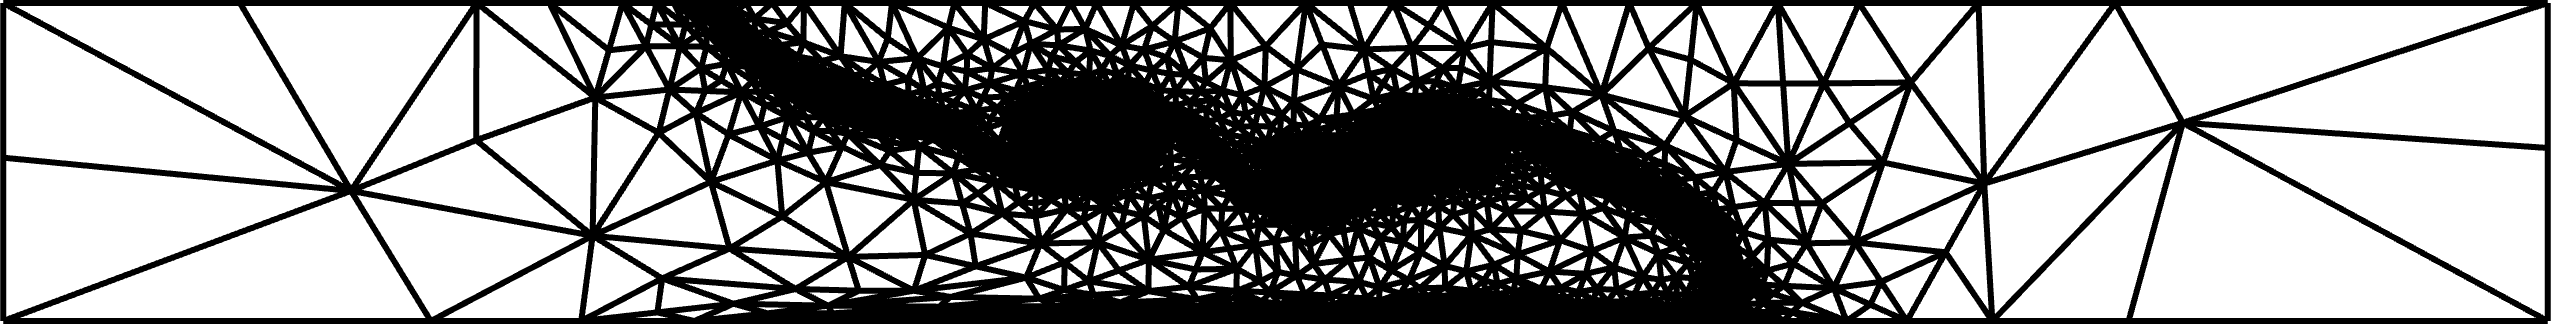
\includegraphics[width=0.45\textwidth]{./lock_exchange/le_basic_10_mesh}} \\
  \subfigure[$t = 37.475\,$s]{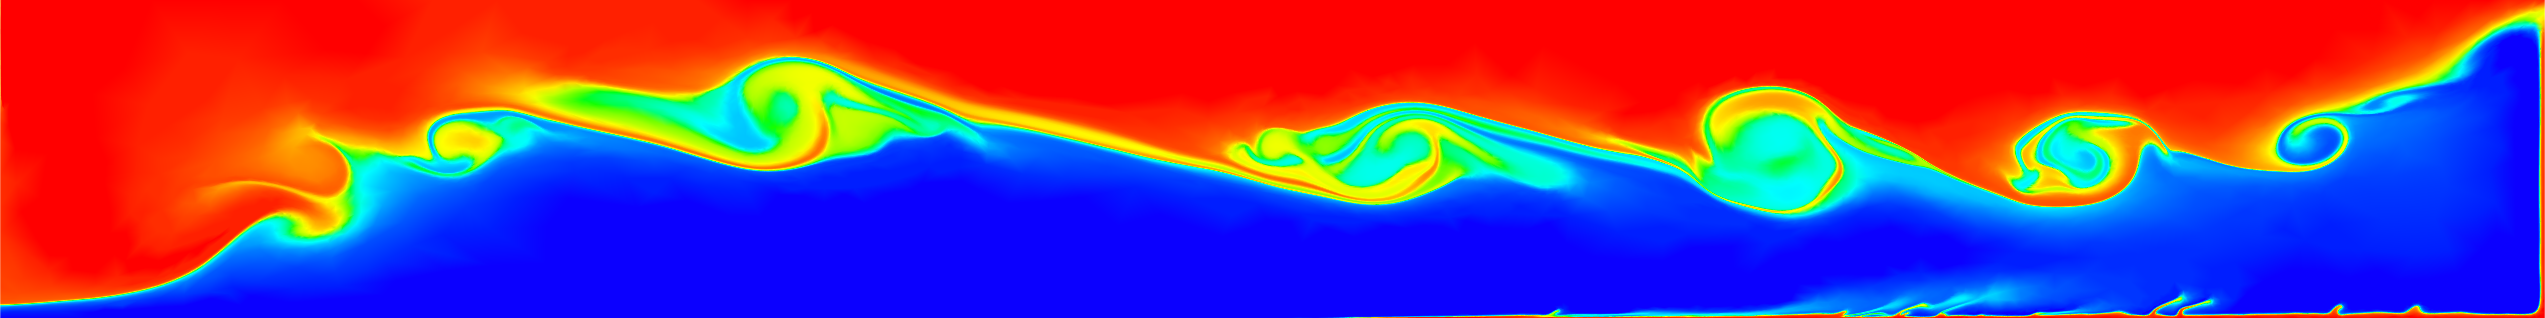
\includegraphics[width=0.45\textwidth]{./lock_exchange/le_basic_30_T}}
  \subfigure[$t =
  37.475\,$s]{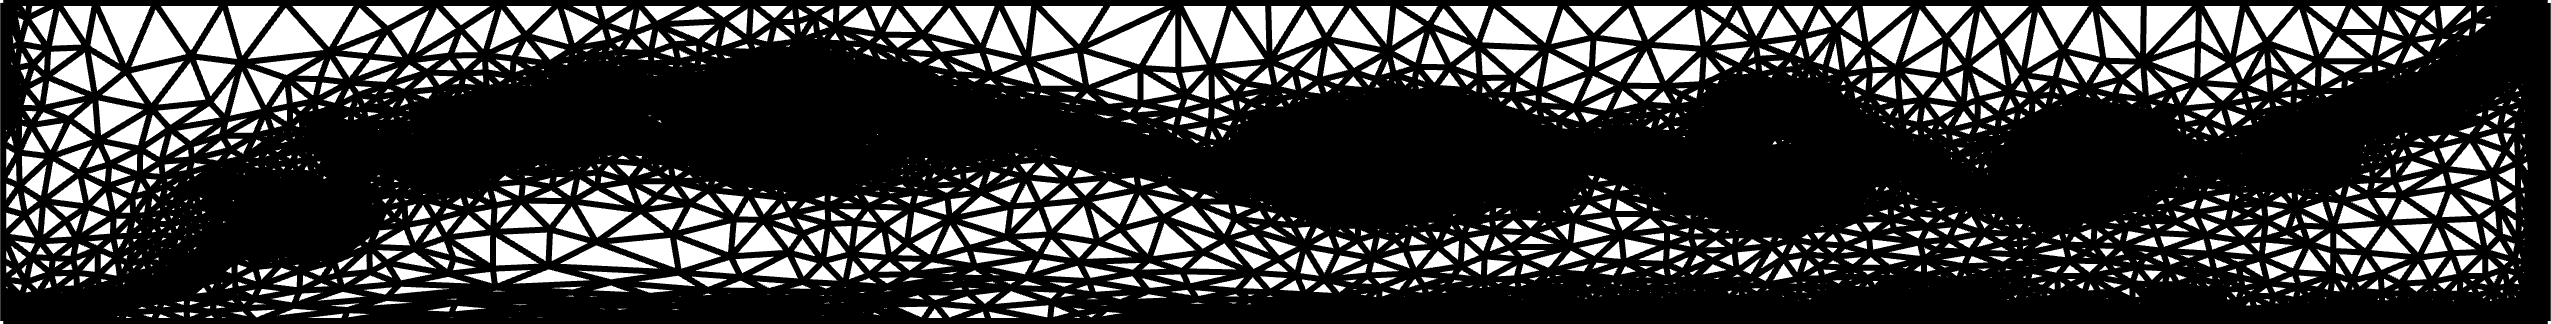
\includegraphics[width=0.45\textwidth]{./lock_exchange/le_basic_30_mesh}}
  \caption{Lock-exchange temperature distribution (colour) with meshes, over time ($t$).}
\end{figure}
\end{frame}
%
\begin{frame}
    \frametitle{The lock--exchange, diagnostics}
\begin{itemize}
\item Front speed (or Froude number)
\item Mixing given by domain fraction of fluid in specified temperature classes
\end{itemize}

\begin{figure}
\centering
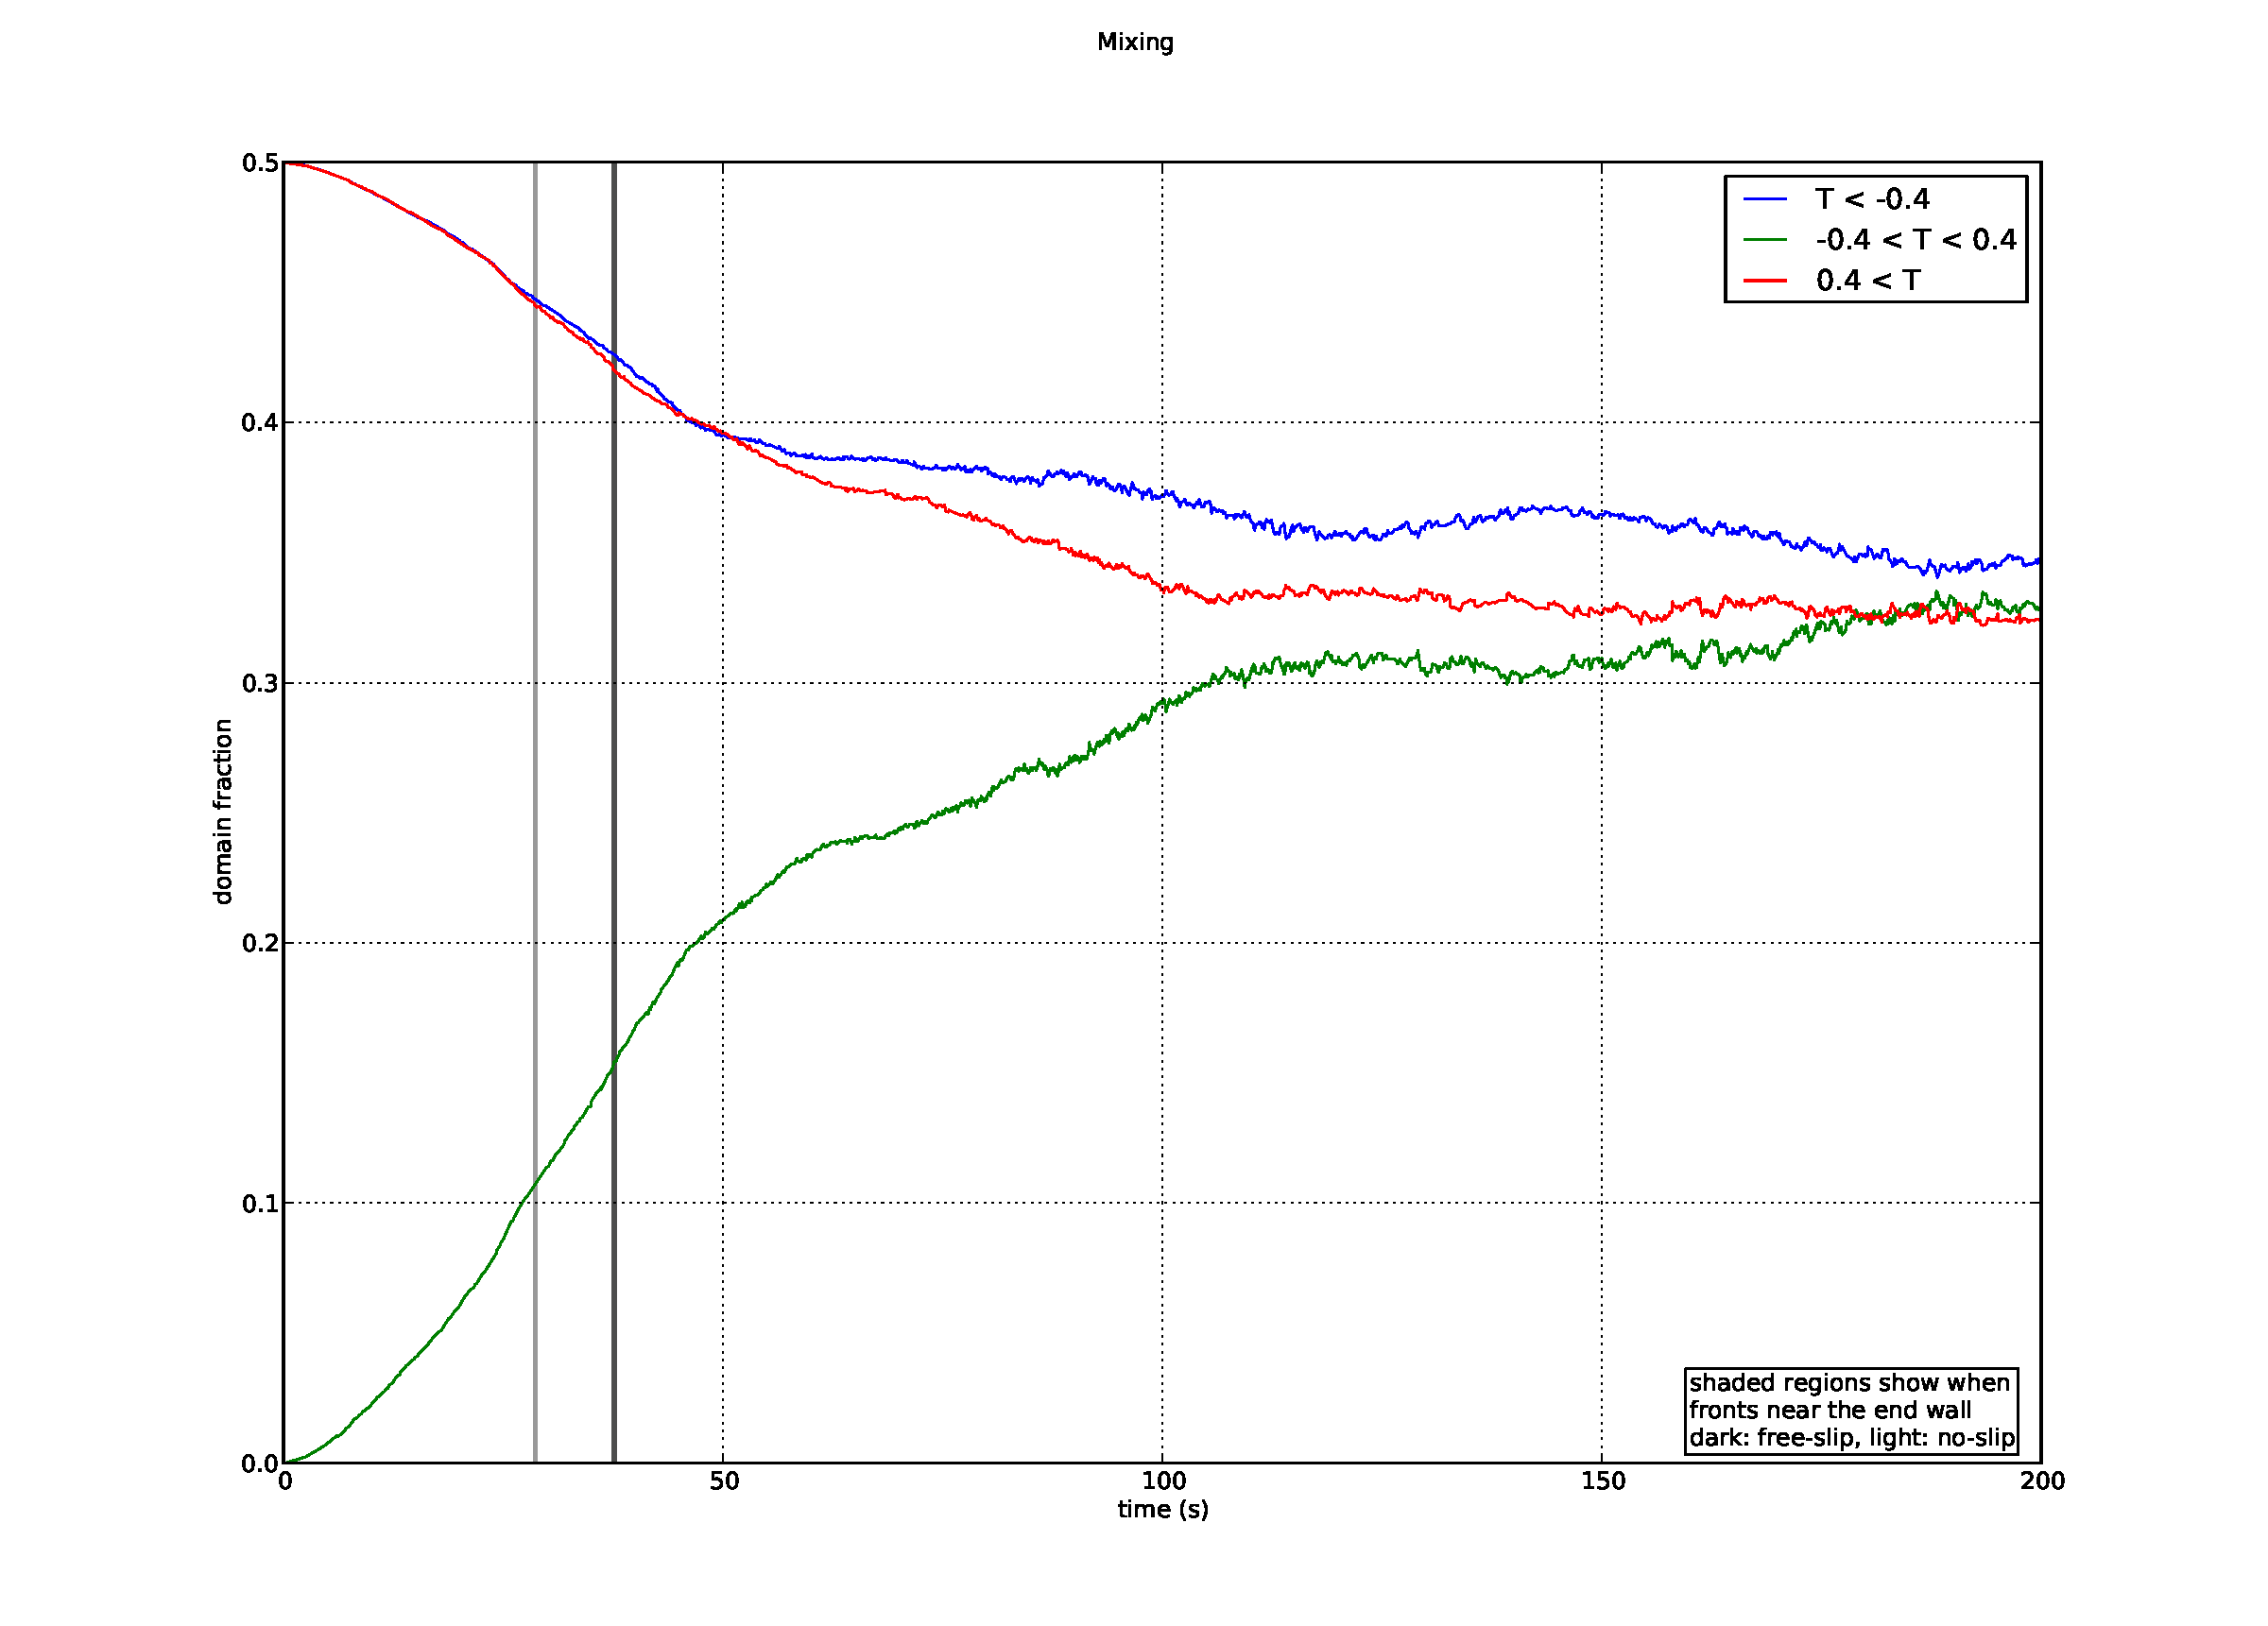
\includegraphics[width=0.5\textwidth]{./lock_exchange/mixing}
\caption{Time evolution of fraction of domain that contains fluid in three temperature classes. Blue: cold, red: warm, green : mixed}
\end{figure}

\end{frame}
%
\begin{frame}
    \frametitle{The lock--exchange, exercises}
\begin{itemize}
\item Increase the simulation time from the default settings (to e.g. 30 secs) and calculate the average Froude number
\item Play with the adaptivity options.
\item Change the diffusivity and viscosity values.
\item Run with a fixed mesh (this will require making a new input mesh)
\item Try adding some detectors to visualise the particle trajectories.
\end{itemize}

\end{frame}
